\section{Investigate important steps in algorithm}
\label{sec:pruning}

\subsection{\leo{Cycle Complexity and Performance}}

In this Section we compare different types of cycles and study how the number
of \textit{Relaxation} steps influence MG's convergence.  The MG algorithm
makes use of many different input parameters that have an impact on its
success.  In our context, we define a strategy as a combination of values of
the most relevant parameters: The type of cycle (V or W), the number of
relaxation steps $\alpha$, and the total number of coarseness levels of the
grid.

%In this context, the MG algorithm makes use of many different input parameters
%such as the iterative method used, the type of cycle and its number of
%repetitions, the number of \textit{Relaxation} at each level or the number of
%different levels to define.

%In this subsection we focus on comparing different types of cycles and study
%how the number of \textit{Relaxation} steps influence the convergence of the
%algorithm.

%We consider 2 types of cycles: the V-cycle and the W-cycle.  The main
%difference between them is that in the W-cycle the recursive call to a coarser
%grid is made twice instead of one before going back to a finer level.

%We call these cycles V-cycle and W-cycle because of how we can draw them if we
%represent each time relaxations are done at a level by a point (see
%Figure~\ref{fig.cycles}).  Figure~\ref{fig.cycles} shows a representation of
%the V- and the W-cyles.  It is possible to define other types of cycles by
%adding more and more repeats of these steps (do $k$ times those steps) to
%generalize the notion of cycle to a $k$-cycle (where a V-cycle is a $1$-cycle
%and a W-cycle is a $2$-cycle).



%The default implementation of BomerAMG does not allow to have different values
%for $\alpha_1,\alpha_2,\dots$ so we set them all to this value $\alpha$.

\begin{table}[hbt]
 \begin{center}
  \begin{tabular}{|c|c|c|c|c|c|c|c|c|}
   \hline
   Type of cycle & V & V & V & V & W & W & W & W \\
   \hline
   $\alpha$ & 1 & 2 & 3 & 10 & 1 & 2 & 3 & 10 \\
   \hline
  \end{tabular}
 \end{center}
 \caption{Combining $\alpha$ and V/W cycles.}
 \label{table.strat1}
\end{table}

We consider a total of 8 different strategies shown in Table~\ref{table.strat1}
where we test V- and W-cycles and we perform 1, 2, 3 and 10 relaxation steps
for each kind of cycle.  For all configurations, the number of different
coarseness levels of the grid is 8.  To compare the different strategies we
consider an input matrix of size $512000 \times 512000$, and a maximum number
of cycles from 1 to 100.  The algorithm's tolerance is set to $0$ to always
reach the maximum number of cycles (1 to 100 depending on the experiments). We
measure for each experiment the final relative residual norm and the execution
time. Each experiment is run 10 times to have an accurate average execution
time.

\begin{figure*}
    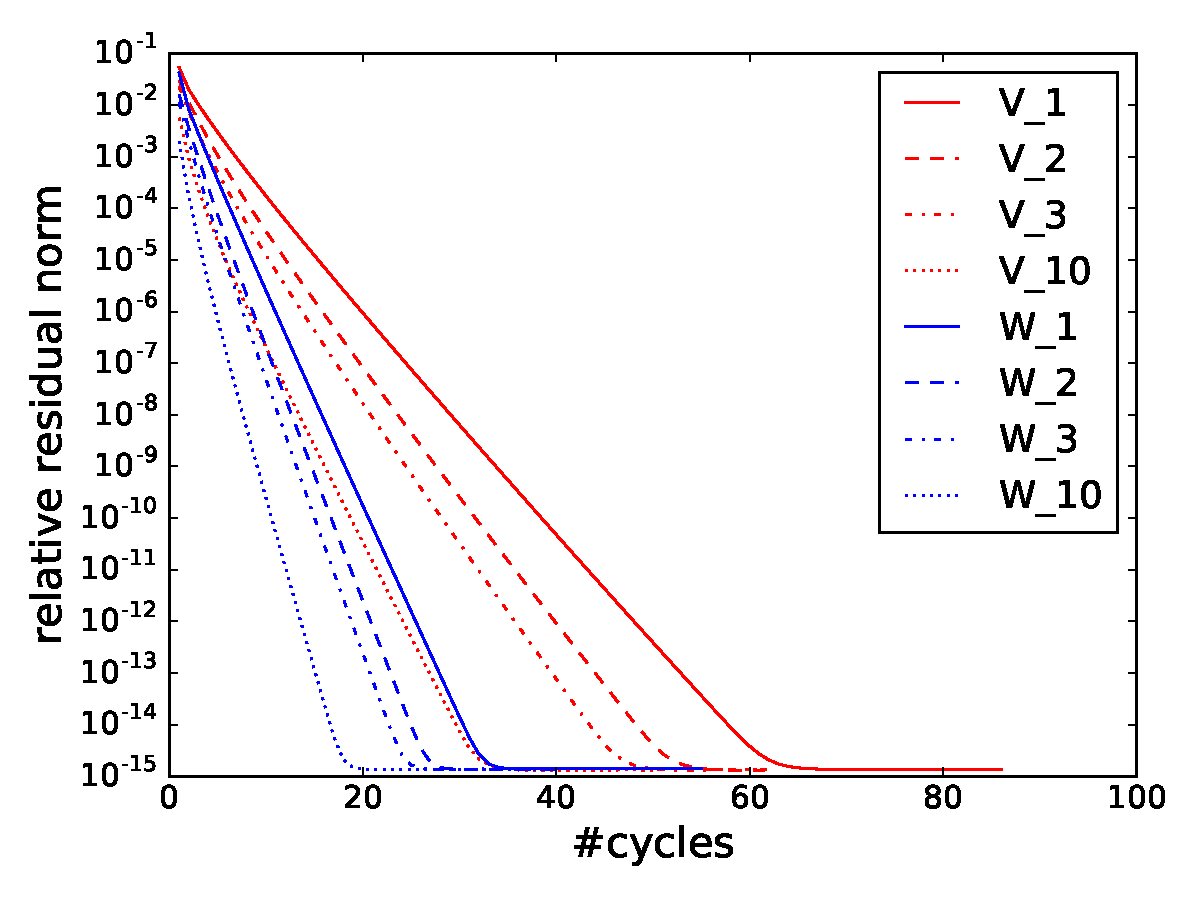
\includegraphics[width=0.33\linewidth]{figs/convergence_1_norm.pdf}
    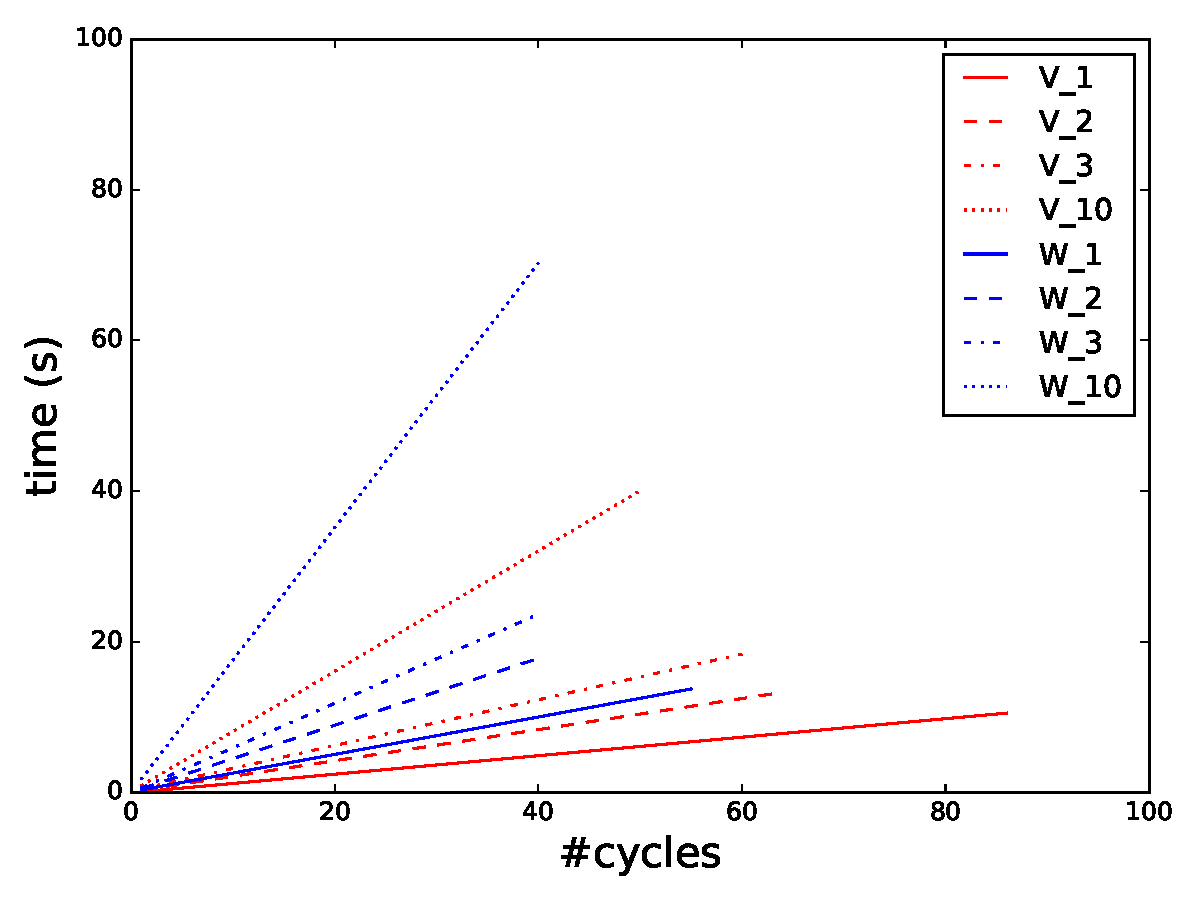
\includegraphics[width=0.33\linewidth]{figs/convergence_1_time.pdf}
    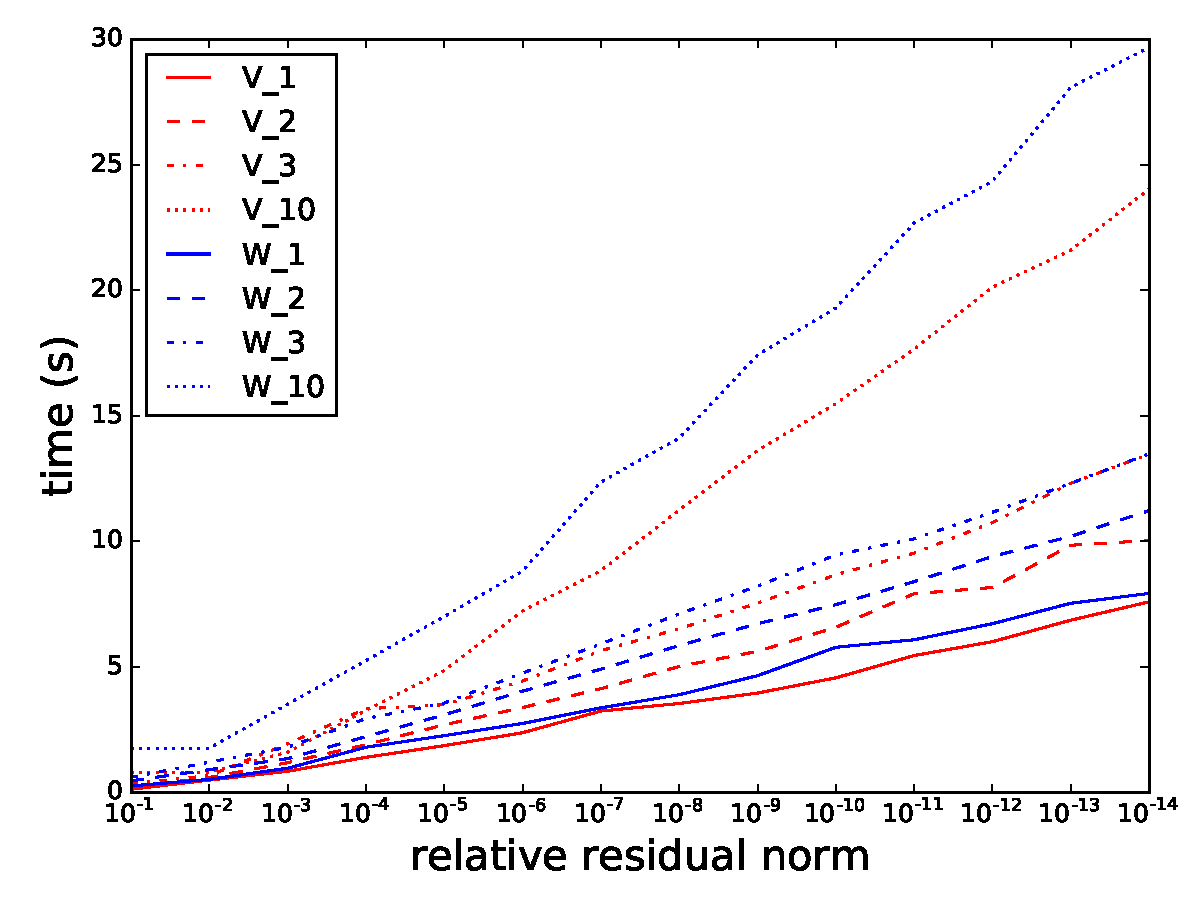
\includegraphics[width=0.33\linewidth]{figs/time_convergence.pdf}
    \caption{Final residual norm of the 8 strategies per iteration (left),
    interpolated execution time per iteration (middle) and convergence time as
    a function of the tolerance (right).}
  \label{fig.first_tests}
\end{figure*}

The results are presented on Figure~\ref{fig.first_tests}.  The left figure
shows how the accuracy evolves with the number of cycles performed.  For
example, we see that the V cycle with 1 relaxation step (plain line in red)
converges with more cycles than the other strategies. However, if we look at
the middle figure we observe that this configuration converges faster than the
other methods.  \leo{This makes sense as the first configuration is a simple
V-cycle with only one relaxation, thus even when the execution requires more
cycles, each cycle is less time consuming and therefore the total execution
time is shorter.}

To be able compare the convergence speed, we present the cost of reaching a
given accuracy on the right figure (left of the x-axis is a small tolerance
i.e.  correspond to accurate results while the right of the x-axis represent
inaccurate (but fast) results). What we can observe is that, as expected,
increasing the number of relaxation steps (i.e., complexifying the cycle)
decreases the number of cycles needed for convergence but it increases the
overall time to do one cycle. We see on the right figure that actually, for a
given precision, the simple V-cycle with only 1 relaxation at each step is the
fastest way to reach it, followed closely by the W-cycle with $\alpha=1$.

The conclusion is that relaxation steps seem to be too costly for the accuracy
they grant. It is better to do more cycles, thus more moves in the grid, than
doing more relaxation steps. This, once again, demonstrates that MG algorithms
are faster than classic iterative methods.


